% !TeX root = RJwrapper.tex
\title{Limitations in Detecting Multicollinearity due to Scaling Issues in the mcvis Package}
\author{by Roman Salmeron Gomez, Catalina B. Garcia Garcia, Ainara Rodriguez Sanchez, and Claudia Garcia Garcia}

\maketitle

\abstract{%
Transformation of the observed data is a very common practice when a troubling degree of near multicollinearity is detected in a linear regression model. However, it is important to take into account that these transformations may affect the detection of this problem, so they should not be performed systematically. In this paper we analyze the transformation of the data when applying the R package mcvis, showing that it only detects essential near multicollinearity when the \emph{studentise} transformation is performed.
}

\hypertarget{introduction}{%
\section{Introduction}\label{introduction}}

Given the model \(\mathbf{Y} = \mathbf{X} \cdot \boldsymbol{\beta} + \mathbf{u}\) for \(n\) observations and \(p\) independent variables where \(\mathbf{Y}\) is a vector that contains the observations of the dependent variables, \(\mathbf{X} = [\mathbf{1} \ \mathbf{X}_{2} \dots \mathbf{X}_{p}]\) is a matrix whose columns contain the observations of the independent variables (where the first column is a vector of ones representing the intercept) and \(\mathbf{u}\) represents the spherical random disturbance, the existence of linear relationships between the independent variables of a model is known as multicollinearity. It is well-known that a high degree of multicollinearity can affect the analysis of a linear regression model. In this case, it is said that the multicollinearity is troubling (Novales 1988; Ramanathan 2002; Wooldridge 2008; Gujarati 2010). It is also interesting to note the distinction made, for example, by Marquardt (1980) or Snee and Marquardt (1984), between essential (near-linear relationship between at least two independent variables excluding the intercept) and non-essential multicollinearity (near-linear relationship between the intercept and at least one of the remaining independent variables).

Note that the detection process is key to determining which tool is best suited to mitigation of the problem: for example, ridge regression of Hoerl and Kennard (1970) and Hoerl and Kennard (1970); LASSO of Tibshirani (1996) or elastic net of Zou and Hastie (2005), among others.

The most commonly applied measures to detect whether the degree of multicollinearity is troubling are the following:

\begin{itemize}
\tightlist
\item
  The Variation Inflation Factor (VIF) that is obtained with the following expression \(VIF(j) = \frac{1}{1-R_{j}^{2}}\), \(j=2,\dots,p\), where \(R_{j}^{2}\) is the coefficient of determination of the auxiliary regression \(\mathbf{X}_{j} = \mathbf{X}_{-j} \cdot \boldsymbol{\alpha} + \mathbf{w}\) with \(\mathbf{X}_{-j}\) being the matrix obtained when the independent variable \(\mathbf{X}_{j}\) is eliminated from matrix \(\mathbf{X}\). It is considered that values of VIF higher than 10 indicate that the degree of multicollinearity is troubling (see, for example, Marquardt (1970) or O'Brien (2007)). Salmerón et al. (2018a) and Salmerón et al. (2020b) showed that the VIF is not an appropriate measure to detect linear relations between the intercept and other explanatory variables (non-essential collinearity).
\item
  The Condition Number (CN) that is obtained with the following expression \(CN(\mathbf{X}) = \sqrt{\frac{\mu_{max}}{\mu_{min}}}\) where \(\mu_{max}\) and \(\mu_{min}\) are the maximum and minimum eigenvalue of matrix \(\mathbf{X}^{t} \mathbf{X}\). To obtain the eigenvalues, the matrix \(\mathbf{X}\) has to be previously transformed in order to ensure that all its columns present unit length (see Salmerón et al. (2018a) for more details about this transformation). Values lower than 20 imply light collinearity, between 20 and 30 moderate collinearity, while values higher than 30 imply strong collinearity (see, for example, Belsley et al. (1980) and Belsley (1991)).
  Another alternative is to calculate the CN with and without the intercept with the goal of analyzing the contribution of the intercept.
\end{itemize}

Another set of measures to detect the existence of troubling multicollinearity are the matrix of simple linear correlations between the independent variables, \(\mathbf{R} = \left( cor(X_{l}, X_{m}) \right)_{l,m=2,\dots,p}\) and its determinant, \(| \mathbf{R} |\).
García et al. (2019) show that values for the coefficient of simple correlation between the independent variables higher than \(\sqrt{0.9}\) and determinant lower than \(0.1013 + 0.00008626 \cdot n - 0.01384 \cdot p\) indicate a troubling degree of multicollinearity (see Salmerón et al. (2021a) or Salmerón et al. (2021b) for more details).
The first value differs strongly from the threshold normally proposed equal to 0.7 to indicate a problem of near collinearity (see, for example, Halkos and Tsilika (2018)).

Also useful to use the coefficient of variation (CV), values less than 0.1002506 indicate the existence of troubling multicollinearity (see Salmerón et al. (2020b) for more details).

García et al. (2016) and Salmerón et al. (2020a) showed that the VIF is invariant to origin and scale changes, which is the same as saying that model \(\mathbf{Y} = \mathbf{X} \cdot \boldsymbol{\beta} + \mathbf{u}\) and the model \(\mathbf{Y} = \mathbf{x} \cdot \boldsymbol{\beta} + \mathbf{u}\) present the same VIF, where \(\mathbf{x} = [\mathbf{x}_{1} \ \mathbf{x}_{2} \dots \mathbf{x}_{p}]\) with \(\mathbf{x}_{i} = \frac{\mathbf{X}_{i}-a_{i}}{b_{i}}\) for \(a_{i} \in \mathbb{R}\), \(b_{i}>0\) and \(i=1,\dots,p\). Note that if \(a_{i} = \overline{\mathbf{X}}_{i}\), \(\mathbf{x}_{1}\) is a vector of zeros, i.e.~the intercept disappears from the model. Instead, Salmerón et al. (2018b) showed that the CN is not invariant to origin and scale changes, meaning that the two previous models present different CNs. This fact implies that models \(\mathbf{Y} = \mathbf{X} \cdot \boldsymbol{\beta} + \mathbf{u}\) and \(\mathbf{Y} = \mathbf{x} \cdot \boldsymbol{\beta} + \mathbf{u}\) present different eigenvalues.

Consequently, transforming the data in a linear regression model may affect the detection of the multicollinearity problem depending on the diagnostic measure. Furthermore, note that this sensitivity to scaling is due to the fact that there are certain transformations (such as data centering) that mitigate the multicollinearity problem, so that the dependence or otherwise on scaling simply highlights the capacity/incapacity of each measure to detect this reduction of the degree of near multicollinearity.

Therefore, when transforming the data in a linear regression model and analyzing whether the degree of multicollinearity is of concern or not, it is necessary to be clear whether the measure used to detect it is affected by the transformation and whether it is capable of detecting the two types of near multicollinearity mentioned (essential and non-essential). Thus, in this paper we analyze the MC index recently presented in Lin et al. (2020).

First, this paper will briefly review the MC index. In order to show that the MC index depends on the transformation of the data and its inability to detect non-essential multicollinearity, we present two simulations with a troubling degree of essential and non-essential multicollinearity, respectively, and a third simulation where the degree of multicollinearity is not troubling. For all these cases, we calculate the different measures to detect multicollinearity commented on the introduction together with the MC index. Two empirical applications recently applied in the scientific literature are also presented. After a discussion of the results we propose a scatter plot between the VIF and CV to detect which variables are the cause of the troubling degree of multicollinearity and the kind of multicollinearity (essential or non-essential) existing in the model. Finally, the main conclusions of the paper are summarized.

\hypertarget{background-mc-index}{%
\section{Background: MC Index}\label{background-mc-index}}

The MC index presented in Lin et al. (2020) is based on the existing relation between the VIFs ant the inverse of the eigenvalues of the matrix \(\mathbf{Z}^{t} \mathbf{Z}\) where \(\mathbf{Z}\) represents the standardized matrix of \(\mathbf{X}\). This is to say, is the matrix \(\mathbf{x}\) mentioned in the introduction when for all \(i\) it is obtained that \(a_{i} = \overline{\mathbf{X}}_{i}\) and \(b_{i} = \sqrt{n \cdot var \left( \mathbf{X}_{i} \right)}\) where \(var \left( \mathbf{X}_{i} \right)\) represents the variance of \(\mathbf{X}_{i}\).
More precisely, taking into account the fact that in the main diagonal of \(\left( \mathbf{Z}^{t} \mathbf{Z} \right)^{-1}\) we find the VIFs (for standardized data), it is possible to establish the following relation:

\begin{equation}
\left(
\begin{array}{c}
VIF(2) \\
\vdots \\
VIF(p)
\end{array}
\right) = \mathbf{A} \cdot \left(
\begin{array}{c}
\frac{1}{\mu_{2}} \\
\vdots \\
\frac{1}{\mu_{p}}
\end{array}
\right),
\end{equation}

where \(\mathbf{A}\) is a matrix that depends on the eigenvalues of \(\mathbf{Z}^{t} \mathbf{Z}\) and \(\mu_{p}\) is the maximum eigenvalue of this matrix.

From this relationship, resampling and obtaining the regression of \(1/\mu_{p}\) as a function of the VIFs, Lin et al. (2020) proposed the use of the t-statistics to conclude which variable contributes the most to this relationship, thus identifying which variables are responsible for the degree of approximate multicollinearity in the model. These authors defined the MC index as \emph{an index from zero to one, larger values indicating greater contribution of the variable i in explaining the observed severity of multicollinearity}.

Taking into account that the calculation of the MC index is based on the relation established between the VIFs and the inverse of the smallest eigenvalue, it seems logical to consider that the transformation of the data may affect the calculation of this measure. Thus, it is possible to conclude:

\begin{itemize}
\tightlist
\item
  If the MC index is calculated with a transformation of the data that leads to the elimination of the intercept, the non-essential multicollinearity will be ignored.
\item
  Due to the fact that MC index is based on the VIF, it should inherit its inability to detect the non-essential multicollinearity.
\end{itemize}

In conclusion, regardless of whether the data is transformed or not, the MC index is not capable of detecting non-essential multicollinearity. It is expected that it will show its usefulness in the case of essential multicollinearity.

Therefore, when Lin et al. (2020) commented that \emph{there are different views on what centering technique is most appropriate in regression {[}\ldots{]} To facilitate this diversity of opinion, in the software implementation of mcvis, we allow the option of passing matrices with different centering techniques as input. The role of scaling is not the focus of our work as our framework does not rely on any specific scaling method}, far from facilitating the use of their proposal, they consider scenarios for which the MC index is not designed, since in their theoretical development and step 2 of their method, the standardization of the data is performed. However, as shown in this paper, the MC index is capable of detecting multicollinearity of the essential type only when used with its default option \emph{studentise}.

\hypertarget{simulations}{%
\section{Simulations}\label{simulations}}

In this section, different versions of the matrix \(\mathbf{X} = [\mathbf{1} \ \mathbf{X}_{2} \ \mathbf{X}_{3} \ \mathbf{X}_{4}]\) will be simulated. The results on the correlation matrix, its determinant, condition number (with and without intercept), variance inflation factor and coefficient of variation are obtained using the \CRANpkg{multiColl} package (see Salmerón et al. (2021a) and Salmerón et al. (2021b) for more details).

In all cases, are calculated the values for the MC index for each set of simulated data considering the two alternative transformation for the data: \emph{euclidean} (centered by mean and divided by Euclidean length) and \emph{studentise} (centered by mean and divided by standard deviation). In each case (simulation and kind of transformation), the calculation of the MC index was performed 100 times.

\hypertarget{simulation-1}{%
\subsection{Simulation 1}\label{simulation-1}}

In this case, 100 observations are generated according to \(\mathbf{X}_{i} \sim N(10, 100)\), \(i=2,3\), and \(\mathbf{X}_{4} = \mathbf{X}_{3} - \mathbf{p}\) where \(\mathbf{p} \sim N(1, 0.5)\). The goal of this simulation is to ensure that the variables \(\mathbf{X}_{3}\) and \(\mathbf{X}_{4}\) will be highly correlated (essential multicollinearity). This fact is confirmed when taking into account the following results in relation to the correlation matrix, correlation matrix's determinant, the CN with and without the intercept (with its corresponding increasing), the VIFs and the coefficient of variation of the different variables.

\begin{verbatim}
  RdetR(X_S1)
\end{verbatim}

\begin{verbatim}
#> $`Correlation matrix`
#>             X2_S1      X3_S1       X4_S1
#> X2_S1  1.00000000 -0.0875466 -0.09110579
#> X3_S1 -0.08754660  1.0000000  0.99881845
#> X4_S1 -0.09110579  0.9988184  1.00000000
#> 
#> $`Correlation matrix's determinant`
#> [1] 0.002330192
\end{verbatim}

\begin{verbatim}
  CNs(X_S1)
\end{verbatim}

\begin{verbatim}
#> $`Condition Number without intercept`
#> [1] 38.67204
#> 
#> $`Condition Number with intercept`
#> [1] 66.94135
#> 
#> $`Increase (in percentage)`
#> [1] 42.22997
\end{verbatim}

\begin{verbatim}
  VIF(X_S1)
\end{verbatim}

\begin{verbatim}
#>      X2_S1      X3_S1      X4_S1 
#>   1.013525 425.587184 425.860062
\end{verbatim}

\begin{verbatim}
  CVs(X_S1)
\end{verbatim}

\begin{verbatim}
#> [1] 1.239795 1.052896 1.166335
\end{verbatim}

Table \ref{tab:Simulation1randomlatex} shows three random iterations, the average value of the 100 times and the standard deviation. As expected in the case of essential multicollinearity, from the average values of Simulation 1 it is noted that (specially with the transformation \emph{studentise}) the MC index correctly identified that the variables \(\mathbf{X}_{3}\) and \(\mathbf{X}_{4}\) are causing the troubling degree of essential multicollinearity. However, it is noted that in some cases the intercept or the variable \(\mathbf{X}_{2}\) are identified as relevant in the existing linear relations when the \emph{euclidean} transformation is performed. This behavior is not observed when the \emph{studentise} transformation is performed. This fact seems to indicate that the MC index depends on the transformation with the \emph{studentise} transformation being the most appropriate.

\begin{table}

\caption{\label{tab:Simulation1randomlatex}MC index for Simulation 1. Three random iterations, the average value of the 100 times and the standard deviation for euclidian and studentise transformations.}
\centering
\begin{tabular}[t]{l|c|c|c}
\hline
  & X2 & X3 & X4\\
\hline
Euclidean - Random 1 & 0.2846628 & 0.3670736 & 0.3482636\\
\hline
Euclidean - Random 2 & 0.1466484 & 0.4444270 & 0.4089246\\
\hline
Euclidean - Random 3 & 0.4026253 & 0.3140131 & 0.2833616\\
\hline
Euclidean - Average & 0.2505292 & 0.3899482 & 0.3595226\\
\hline
Euclidean - Standard Deviation & 0.1075164 & 0.0550333 & 0.0526817\\
\hline
Studentise - Random 1 & 0.0000338 & 0.4942761 & 0.5056901\\
\hline
Studentise - Random 2 & 0.0001294 & 0.4901233 & 0.5097473\\
\hline
Studentise - Random 3 & 0.0000307 & 0.4950536 & 0.5049157\\
\hline
Studentise - Average & 0.0000519 & 0.4944290 & 0.5055191\\
\hline
Studentise - Standard Deviation & 0.0000264 & 0.0023510 & 0.0023528\\
\hline
\end{tabular}
\end{table}

\hypertarget{simulation-2}{%
\subsection{Simulation 2}\label{simulation-2}}

In this case, 100 observations are generated according to \(\mathbf{X}_{i} \sim N(10, 100)\), \(i=2,3\), and \(\mathbf{X}_{4} \sim N(10, 0.0001)\). The goal of this simulation is to ensure that the variable \(\mathbf{X}_{4}\) will be highly correlated to the intercept (non-essential multicollinearity). This fact is confirmed from the following results taking into account that Salmerón et al. (2020b) showed that a value of the CV lower than 0.1002506 indicates a troubling degree of non-essential multicollinearity.

\begin{verbatim}
RdetR(X_S2)
\end{verbatim}

\begin{verbatim}
#> $`Correlation matrix`
#>            X2_S2       X3_S2      X4_S2
#> X2_S2  1.0000000 -0.08754660 0.06676070
#> X3_S2 -0.0875466  1.00000000 0.09445547
#> X4_S2  0.0667607  0.09445547 1.00000000
#> 
#> $`Correlation matrix's determinant`
#> [1] 0.9778526
\end{verbatim}

\begin{verbatim}
CNs(X_S2)
\end{verbatim}

\begin{verbatim}
#> $`Condition Number without intercept`
#> [1] 2.999836
#> 
#> $`Condition Number with intercept`
#> [1] 2430.189
#> 
#> $`Increase (in percentage)`
#> [1] 99.87656
\end{verbatim}

\begin{verbatim}
VIF(X_S2)
\end{verbatim}

\begin{verbatim}
#>    X2_S2    X3_S2    X4_S2 
#> 1.013525 1.018091 1.014811
\end{verbatim}

\begin{verbatim}
CVs(X_S2)
\end{verbatim}

\begin{verbatim}
#> [1] 1.239794695 1.052896496 0.001022819
\end{verbatim}

Table \ref{tab:Simulation2randomlatex} presents three random iterations, the average value of the 100 times and the standard deviation for Simulation 2 for \emph{euclidian} and \emph{studentise} transformations. Before commenting the results of Simulation 2, it is important to take into account the fact that with transformations that imply the elimination of the intercept it will not be possible to detect the non-essential multicollinearity.
Note that in some occasions, when \emph{euclidean} transformation is performed, it is concluded that \(\mathbf{X}_{3}\) and \(\mathbf{X}_{4}\) are the most relevant while, when \emph{studentise} transformation is performed, all variables seem to present the same relevance. In the first case, a higher stability is observed by considering the average values, although the conclusion is that there is a relation between \(\mathbf{X}_{3}\) and \(\mathbf{X}_{4}\) when the relationship is between the intercept and \(\mathbf{X}_{4}\).

\begin{table}

\caption{\label{tab:Simulation2randomlatex}MC index for Simulation 2. Three random iterations, the average value of the 100 times and the standard deviation for euclidian and studentise transformations.}
\centering
\begin{tabular}[t]{l|c|c|c}
\hline
  & X2 & X3 & X4\\
\hline
Euclidean - Random 1 & 0.2671991 & 0.2097102 & 0.5230907\\
\hline
Euclidean - Random 2 & 0.1649092 & 0.5119198 & 0.3231711\\
\hline
Euclidean - Random 3 & 0.2126011 & 0.2678652 & 0.5195337\\
\hline
Euclidean - Average & 0.1678676 & 0.3335266 & 0.4986058\\
\hline
Euclidean - Standard Deviation & 0.0725673 & 0.0845660 & 0.1029678\\
\hline
Studentise - Random 1 & 0.3307490 & 0.3342851 & 0.3349658\\
\hline
Studentise - Random 2 & 0.3646487 & 0.2995420 & 0.3358093\\
\hline
Studentise - Random 3 & 0.3107573 & 0.3481032 & 0.3411395\\
\hline
Studentise - Average & 0.3541923 & 0.3150319 & 0.3307758\\
\hline
Studentise - Standard Deviation & 0.0201173 & 0.0203717 & 0.0187872\\
\hline
\end{tabular}
\end{table}

\hypertarget{simulation-3}{%
\subsection{Simulation 3}\label{simulation-3}}

Finally, in this case 100 observations are generated according to \(\mathbf{X}_{i} \sim N(10, 100)\), \(i=2,3,4\). The goal of this simulation is to ensure that the degree of multicollinearity (essential and non-essential) will be not troubling. This fact is confirmed when taking into account the following results.

\begin{verbatim}
RdetR(X_S3)
\end{verbatim}

\begin{verbatim}
#> $`Correlation matrix`
#>            X2_S3       X3_S3      X4_S3
#> X2_S3  1.0000000 -0.08754660 0.06676070
#> X3_S3 -0.0875466  1.00000000 0.09445547
#> X4_S3  0.0667607  0.09445547 1.00000000
#> 
#> $`Correlation matrix's determinant`
#> [1] 0.9778526
\end{verbatim}

\begin{verbatim}
CNs(X_S3)
\end{verbatim}

\begin{verbatim}
#> $`Condition Number without intercept`
#> [1] 2.07584
#> 
#> $`Condition Number with intercept`
#> [1] 3.60862
#> 
#> $`Increase (in percentage)`
#> [1] 42.47552
\end{verbatim}

\begin{verbatim}
VIF(X_S3)
\end{verbatim}

\begin{verbatim}
#>    X2_S3    X3_S3    X4_S3 
#> 1.013525 1.018091 1.014811
\end{verbatim}

\begin{verbatim}
CVs(X_S3)
\end{verbatim}

\begin{verbatim}
#> [1] 1.239795 1.052896 1.019006
\end{verbatim}

Table \ref{tab:Simulation3randomlatex} presents three random iterations, the average value of the 100 times and the standard deviation for Simulation 3 for \emph{euclidian} and \emph{studentise} transformations. Simulation 3 shows different situations depending on the transformation: when the \emph{euclidean} transformation is performed, the variable \(\mathbf{X}_{3}\) is also identified apart from variable \(\mathbf{X}_{4}\); with the \emph{studentise} transformation, all the variables seem to be relevant.

\begin{table}

\caption{\label{tab:Simulation3randomlatex}MC index for Simulation 3. Three random iterations, the average value of the 100 times and the standard deviation for euclidian and studentise transformations.}
\centering
\begin{tabular}[t]{l|c|c|c}
\hline
  & X2 & X3 & X4\\
\hline
Euclidean - Random 1 & 0.1318422 & 0.3832372 & 0.4849206\\
\hline
Euclidean - Random 2 & 0.1679453 & 0.4315253 & 0.4005294\\
\hline
Euclidean - Random 3 & 0.0728076 & 0.5693939 & 0.3577986\\
\hline
Euclidean - Average & 0.1083812 & 0.4107279 & 0.4808910\\
\hline
Euclidean - Standard Deviation & 0.0410296 & 0.0661189 & 0.0628212\\
\hline
Studentise - Random 1 & 0.3586837 & 0.3154482 & 0.3258681\\
\hline
Studentise - Random 2 & 0.3805084 & 0.3205751 & 0.2989166\\
\hline
Studentise - Random 3 & 0.3651891 & 0.3069920 & 0.3278189\\
\hline
Studentise - Average & 0.3541923 & 0.3150319 & 0.3307758\\
\hline
Studentise - Standard Deviation & 0.0201173 & 0.0203717 & 0.0187872\\
\hline
\end{tabular}
\end{table}

\hypertarget{interpretation-of-the-obtained-results}{%
\subsection{Interpretation of the obtained results}\label{interpretation-of-the-obtained-results}}

From the above results, it is concluded that the MC index applied individually is not able to detect if the degree of multicollinearity is troubling. This conclusion is in line with the comment presented by Lin et al. (2020) where it is stated that \emph{those classical collinearity measures are used together with mcvis for the better learning of how one or more variables display dominant behavior in explaining multicollinearity}. That is to say, it is recommended to use measures such as the VIF and the CN to detect whether the degree of multicollinearity is troubling and, if it is, then use the MC index to detect which variables are more relevant.

We should reiterate the fact that the results of the MC index depend on the transformation performed with the data.

Finally, it is worthy of note that the lowest dispersion is obtained when the \emph{studentise} transformation is performed, which indicate that with this transformation a higher stability exists in the results obtained with the 100 iterations performed.

\hypertarget{examples}{%
\section{Examples}\label{examples}}

In this section we will analyze two examples applied recently to illustrate the multicollinearity problem. The first one focuses on the existence of non-essential approximate multicollinearity while the second one is focused on essential multicollinearity.

\hypertarget{example-1}{%
\subsection{Example 1}\label{example-1}}

Salmerón et al. (2020b) analyzed the Euribor as a function of the harmonized index of consumer prices (\textbf{HICP}), the balance of payments to net current account (\textbf{BC}) and the government deficit to net non-financial accounts (\textbf{GD}). See data set in Table \ref{tab:Example1Datalatex}.

\begin{table}

\caption{\label{tab:Example1Datalatex}Data set for example . @Salmeron2020a}
\centering
\begin{tabular}[t]{c|c|c|c}
\hline
Euribor & HIPC & BC & GD\\
\hline
3.63 & 92.92 & 17211 & -51384.0\\
\hline
3.90 & 93.85 & 2724 & -49567.1\\
\hline
3.45 & 93.93 & 17232 & -52128.4\\
\hline
3.01 & 94.41 & 9577 & -53593.3\\
\hline
2.54 & 95.08 & 4117 & -65480.0\\
\hline
2.23 & 95.73 & -2134 & -50343.8\\
\hline
2.20 & 95.90 & 6117 & -75646.4\\
\hline
2.36 & 96.40 & 10949 & -59120.8\\
\hline
2.14 & 96.77 & 18360 & -69246.3\\
\hline
2.29 & 97.97 & 13646 & -60313.8\\
\hline
2.35 & 98.06 & 8424 & -56782.9\\
\hline
2.32 & 98.67 & 14319 & -55313.1\\
\hline
2.32 & 98.76 & 3885 & -67034.4\\
\hline
2.19 & 99.96 & 4493 & -61942.8\\
\hline
2.20 & 100.30 & -320 & -46258.4\\
\hline
2.63 & 100.97 & -2736 & -43761.4\\
\hline
2.95 & 101.07 & -6909 & -37562.6\\
\hline
3.31 & 102.44 & -4848 & -35609.6\\
\hline
3.62 & 102.52 & -4255 & -27064.0\\
\hline
3.60 & 102.79 & 1347 & -32497.2\\
\hline
4.09 & 102.97 & 8781 & -18389.0\\
\hline
4.38 & 104.38 & 8723 & -9923.5\\
\hline
4.65 & 104.45 & 3662 & -9727.0\\
\hline
4.68 & 105.77 & -17548 & -23729.9\\
\hline
4.48 & 106.43 & -37041 & -28909.3\\
\hline
5.05 & 108.18 & -27624 & -46527.0\\
\hline
5.37 & 108.49 & -37723 & -49654.0\\
\hline
4.34 & 108.21 & -43584 & -81729.7\\
\hline
2.22 & 107.46 & -16070 & -121227.5\\
\hline
1.67 & 108.37 & -5029 & -142580.9\\
\hline
1.34 & 108.08 & 7294 & -164699.2\\
\hline
1.24 & 108.67 & 85 & -152269.2\\
\hline
1.22 & 108.67 & -4399 & -162477.4\\
\hline
1.25 & 110.12 & -2431 & -128366.4\\
\hline
1.40 & 109.95 & 2137 & -169848.0\\
\hline
1.52 & 110.87 & -4345 & -129290.2\\
\hline
1.74 & 111.36 & -12643 & -104646.7\\
\hline
2.13 & 113.15 & -2272 & -103143.8\\
\hline
2.11 & 112.91 & -3592 & -102621.8\\
\hline
2.06 & 114.12 & 8071 & -104240.4\\
\hline
1.67 & 114.35 & 12202 & -82309.3\\
\hline
1.28 & 115.93 & 35619 & -91620.9\\
\hline
0.90 & 115.78 & 42161 & -85054.4\\
\hline
0.60 & 116.75 & 43880 & -99998.2\\
\hline
0.57 & 116.47 & 52483 & -81287.1\\
\hline
0.51 & 117.55 & 56376 & -77738.8\\
\hline
0.54 & 117.34 & 48981 & -73003.3\\
\hline
\end{tabular}
\end{table}

The following determinant of the matrix of correlations of the independent variables, the VIFs, condition number without intercept and with intercept and the coefficients of variation indicate that the degree of essential near multicollinearity is not troubling while the non-essential type (due to the variable \textbf{HIPC}) is.

\begin{verbatim}
RdetR(data1)
\end{verbatim}

\begin{verbatim}
#> $`Correlation matrix`
#>            HIPC          BC          GD
#> HIPC  1.0000000  0.23129203 -0.46855433
#> BC    0.2312920  1.00000000 -0.07033647
#> GD   -0.4685543 -0.07033647  1.00000000
#> 
#> $`Correlation matrix's determinant`
#> [1] 0.7372587
\end{verbatim}

\begin{verbatim}
CNs(data1)
\end{verbatim}

\begin{verbatim}
#> $`Condition Number without intercept`
#> [1] 4.259658
#> 
#> $`Condition Number with intercept`
#> [1] 39.35375
#> 
#> $`Increase (in percentage)`
#> [1] 89.17598
\end{verbatim}

\begin{verbatim}
VIF(data1)
\end{verbatim}

\begin{verbatim}
#>     HIPC       BC       GD 
#> 1.349666 1.058593 1.283815
\end{verbatim}

\begin{verbatim}
CVs(data1)
\end{verbatim}

\begin{verbatim}
#> [1] 0.06957876 4.34031035 0.55015508
\end{verbatim}

Figure \ref{fig:Example1-static} shows a tour displayed with a scatterplot by using the \CRANpkg{tourr} package. This package allows tours of multivariate data, see Wickham et al. (2011) for more details. From the tour on all the explanatory variables (it runs for 3.47 minutes in the html version), no linear relation is observed between the explanatory variables. Note that this package does not allow us to work with the intercept.

\begin{figure}
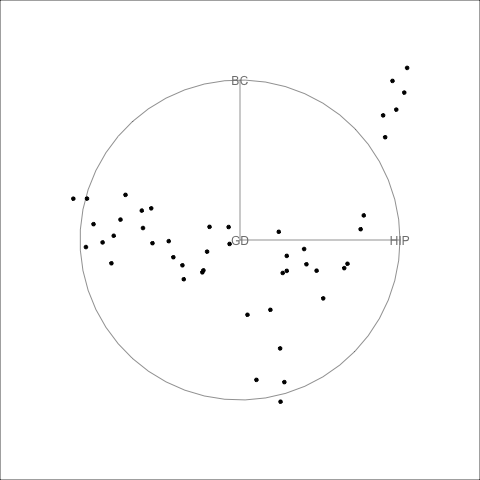
\includegraphics[width=0.5\linewidth]{Example1plot1} 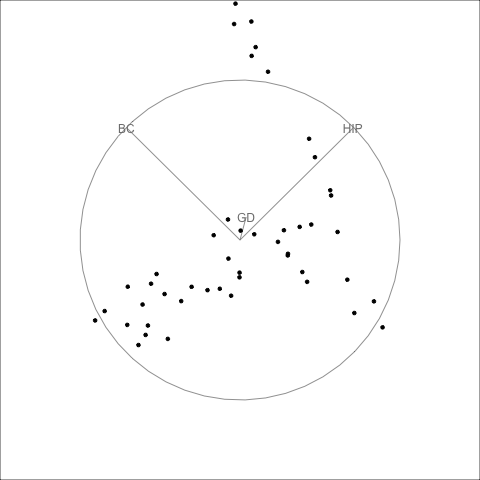
\includegraphics[width=0.5\linewidth]{Example1plot2} 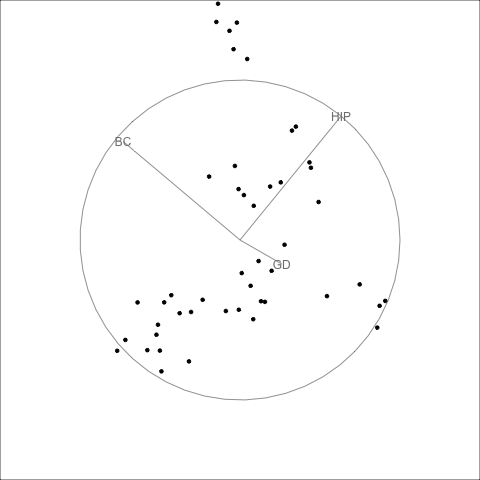
\includegraphics[width=0.5\linewidth]{Example1plot3} 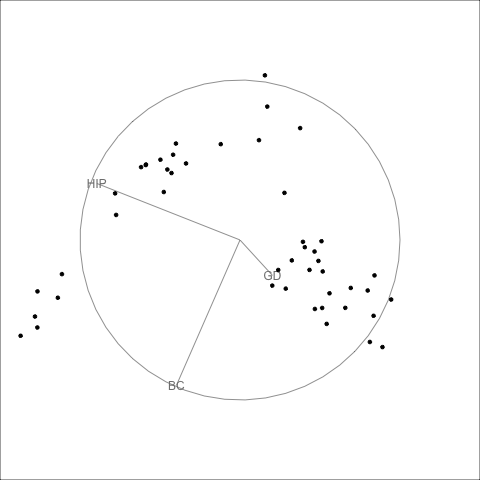
\includegraphics[width=0.5\linewidth]{Example1plot4} \caption{Representation  of example 1 using the R tourr package. No linear relationship is observed between the explanatory variables. See html version for an interactive 2-D tour.}\label{fig:Example1-static}
\end{figure}

In relation to the application of the \CRANpkg{mcvis} package in this example, it can be observed that if the \emph{euclidean} transformation is performed the method concludes that all the variables seem to be relevant:

\begin{verbatim}
#>      HIPC   BC   GD
#> tau3 0.29 0.39 0.32
\end{verbatim}

For \emph{studentise} transformation it concludes the establishing of a relationship between \textbf{HIPC} and \textbf{GD}:

\begin{verbatim}
#>      HIPC   BC   GD
#> tau3 0.49 0.13 0.38
\end{verbatim}

Clearly, these conclusions are not consistent. Moreover, by eliminating the intercept when transforming the data, it is not feasible to detect the non-essential multicollinearity.

\hypertarget{example-2}{%
\subsection{Example 2}\label{example-2}}

James et al. (2013) illustrated multicollinearity with a data set which contains information about the dependent variable \textbf{balance} (average credit card debt for a number of individuals) and, among others, the following quantitative independent variables: \textbf{income}, \textbf{limit} (credit limit), \textbf{rating} (credit rating), \textbf{cards} (number of credit cards), \textbf{age}, \textbf{education} (years of education). Data is available in the \CRANpkg{ISLR} package (see James et al. (2021) for more details).

The following determinant of the matrix of correlations of the independent variables, the simple correlation between \textbf{limit} and \textbf{rating} (0.99687974), the VIFs, condition number without intercept and with intercept and CVs indicate that the degree of approximate multicollinearity of the non-essential type is not troubling while that of the essential type (due to the relationship between variables \textbf{limit} and \textbf{rating}) is troubling.

\begin{verbatim}
RdetR(data2)
\end{verbatim}

\begin{verbatim}
#> $`Correlation matrix`
#>                Income       Limit      Rating       Cards         Age
#> Income     1.00000000  0.79208834  0.79137763 -0.01827261 0.175338403
#> Limit      0.79208834  1.00000000  0.99687974  0.01023133 0.100887922
#> Rating     0.79137763  0.99687974  1.00000000  0.05323903 0.103164996
#> Cards     -0.01827261  0.01023133  0.05323903  1.00000000 0.042948288
#> Age        0.17533840  0.10088792  0.10316500  0.04294829 1.000000000
#> Education -0.02769198 -0.02354853 -0.03013563 -0.05108422 0.003619285
#>              Education
#> Income    -0.027691982
#> Limit     -0.023548534
#> Rating    -0.030135627
#> Cards     -0.051084217
#> Age        0.003619285
#> Education  1.000000000
#> 
#> $`Correlation matrix's determinant`
#> [1] 0.00154733
\end{verbatim}

\begin{verbatim}
CNs(data2)
\end{verbatim}

\begin{verbatim}
#> $`Condition Number without intercept`
#> [1] 109.4461
#> 
#> $`Condition Number with intercept`
#> [1] 128.699
#> 
#> $`Increase (in percentage)`
#> [1] 14.95963
\end{verbatim}

\begin{verbatim}
VIF(data2)
\end{verbatim}

\begin{verbatim}
#>     Income      Limit     Rating      Cards        Age  Education 
#>   2.773276 228.848290 230.612596   1.433932   1.038541   1.008043
\end{verbatim}

\begin{verbatim}
CVs(data2)
\end{verbatim}

\begin{verbatim}
#> [1] 0.7784400 0.4868046 0.4353711 0.4630802 0.3094845 0.2320668
\end{verbatim}

Figure \ref{fig:Example2-static} displays its tour by using again \CRANpkg{tourr} package. Multicollinearity was checked using a tour on all the explanatory variables (it runs for 3.47 minutes in html version). In this case a certain linear relationship is observed, although it is difficult to determine which variables are related.

\begin{figure}
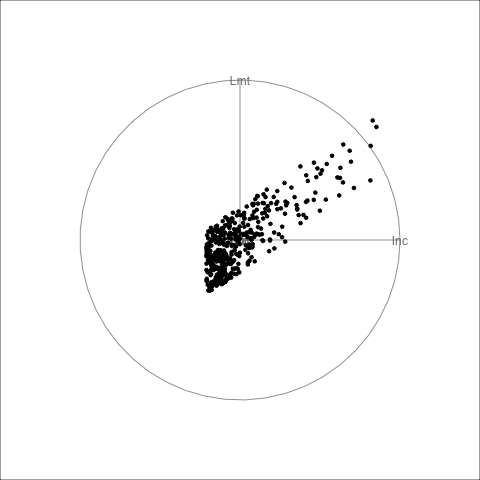
\includegraphics[width=0.5\linewidth]{Example2plot1} 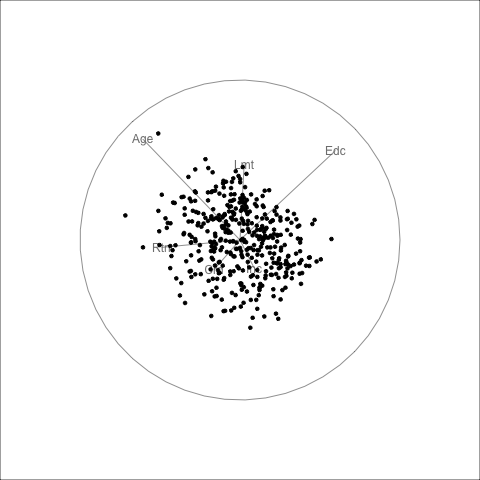
\includegraphics[width=0.5\linewidth]{Example2plot2} 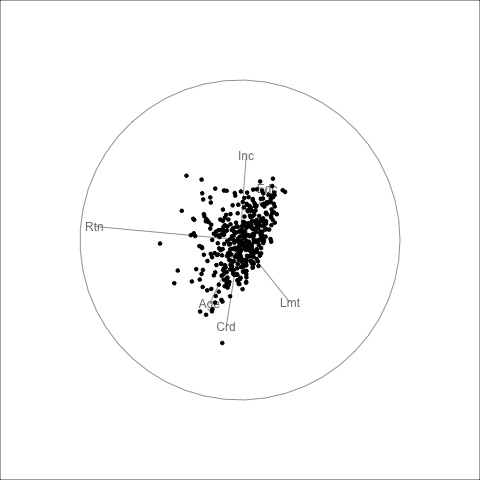
\includegraphics[width=0.5\linewidth]{Example2plot3} 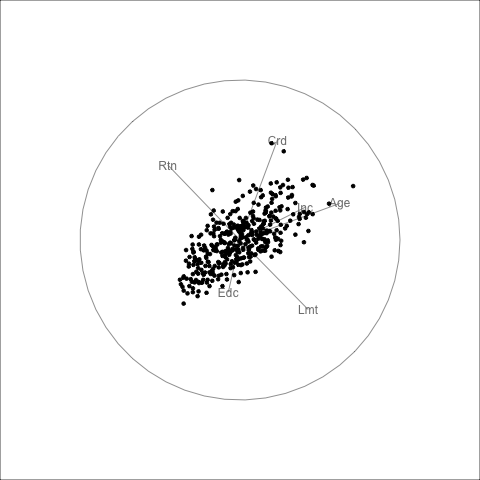
\includegraphics[width=0.5\linewidth]{Example2plot4} \caption{Representation  of example 2 using the R tourr package. A certain linear relationship bewteen independent variables is observed. See html version for an interactive 2-D tour.}\label{fig:Example2-static}
\end{figure}

In relation to the application of the \CRANpkg{mcvis} package in this example, it can be observed that if the \emph{euclidean} transformation is performed the variable with the highest value is \textbf{income}, with the variable \textbf{rating} being the second-lowest in value.

\begin{verbatim}
#>      Income Limit Rating Cards  Age Education
#> tau6   0.62  0.14   0.05  0.05 0.11      0.03
\end{verbatim}

Finally, when the \emph{studentise} transformation is applied, the method clearly indicates that variables \textbf{limit} and \textbf{rating} are the ones responsible for the multicollinearity problem.

\begin{verbatim}
#>      Income Limit Rating Cards Age Education
#> tau6      0  0.49   0.51     0   0         0
\end{verbatim}

\hypertarget{discussion}{%
\section{Discussion}\label{discussion}}

The results shown in the previous sections indicate that, on the one hand, the calculation of the MC index depends on the transformation performed and, on the other hand, that to apply this index with guarantees, the \emph{studentise} transformation is the most appropriate.

It was also showed that the MC index ``inherits'\,' the same limitations indicated by Lin et al. (2020) when they state that \emph{collinearity indices such as the variance inflation factor and the condition number have limitations and may not be effective in some applications}. In the case of VIF, these limitations are well summarized by Lin et al. (2020): \emph{The VIF can show how variables are correlated to each other, but as shown, low correlation does not guarantee low level of collinearity}.
Note that the example applied by the authors in Section 1 (similar to the one presented in Salmerón et al. (2018a) and a reduced version of the one presented by Belsley (1984)) is a clear case in which the multicollinearity is non-essential. As was commented earlier, the VIF ((Salmerón et al. 2018a) and (Salmerón et al. 2020b)) and the MC index are not able to detect this kind of multicollinearity, for this reason they are only recommended for detecting essential multicollinearity.

Another limitation of the VIF (and also of the MC index) worthy of note is that it is not adequate for calculating with dummy variables. Using these kinds of variables, the VIF is obtained from a coefficient of determination of an auxiliary regression whose dependent variable is a dummy variable. Although it is possible to apply ordinary least squares in this kind of regression, it is well known that it can present some problems: for example, the coefficient of determination is not representative since it measures the linear relation but the relation between the dummy variable and the rest of independent variables is not linear. For this reason, these kinds of regressions are estimated with non-linear models such as the logit/probit. Thus, we consider that if it is not adequate for calculating the VIF associated to a dummy variable, these kinds of variables should be avoided in the calculation of the MC index.

Finally, Simulation 3 shows that MC index is not able to detect whether the degree of essential multicollinearity is troubling. For this reason, it should only be used once this situation is determined by other measures (as set out in the introduction) and in order to determine which variables cause it.

\hypertarget{solution}{%
\section{Solution}\label{solution}}

The distinction between essential and non-essential multicollinearity and the limitations of each measure for detecting the different kinds of multicollinearity, can be very useful for detecting whether there is a troubling degree of multicollinearity, what kind of multicollinearity it is and which variables are causing the multicollinearity. Thus, taking into account the fact that the VIF is useful for detecting essential multicollinearity and the CV is useful for detecting non-essential multicollinearity, the scatter plot of both measures can provide interesting information in a joint way.

We present the scatter plot for the values of the VIF and the CV for the three simulations previously performed. Note that the figures include the lines corresponding to the established thresholds for each measure: red dashed vertical line for 0.1002506 (CV) and red dotted horizontal line for 10 (VIF). These lines determine four regions that can be interpreted as follows: A, existence of troubling non-essential and non-troubling essential multicollinearity; B, existence of troubling essential and non-essential multicollinearity; C, existence of non-troubling non-essential and troubling essential multicollinearity; D: non-troubling degree of existing multicollinearity (essential and non-essential).

Considering this classification, in Simulation 1 (Figure \ref{fig:FigureS1}) it is noted that there is a troubling degree of essential multicollinearity due to the variables \(\mathbf{X}_{3}\) and \(\mathbf{X}_{4}\), while in Simulation 2 (Figure \ref{fig:FigureS2}) it is noted that there is a troubling degree of non-essential multicollinearity due to the variable \(\mathbf{X}_{4}\) and in Simulation 3 (Figure \ref{fig:FigureS3}) it is noted that the degree of multicollinearity is not troubling.

\begin{figure}
\centering
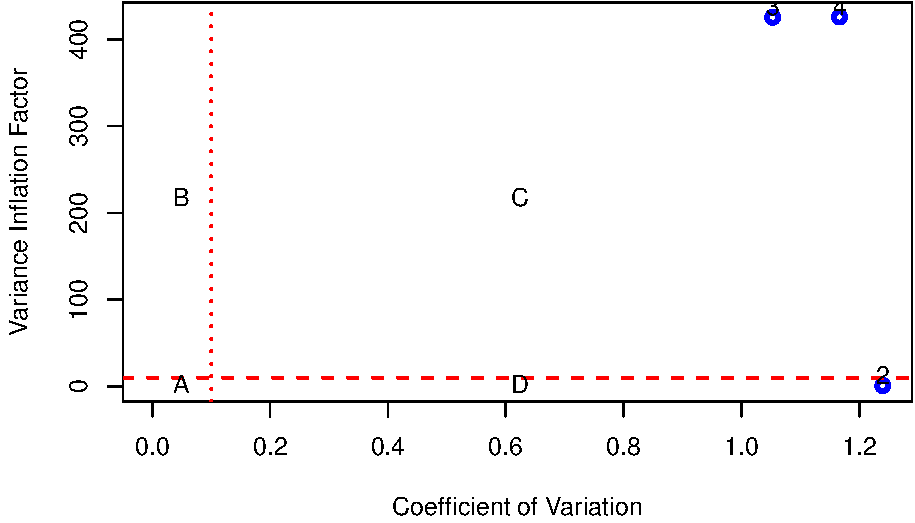
\includegraphics{salmeron-etal_files/figure-latex/FigureS1-1.pdf}
\caption{\label{fig:FigureS1}Representation of the VIFs and CVs of explanatory variables in Simulation 1. A troubling degree of essential multicollinearity due to variables 3 and 4 is detected by considering thresholds of 0.1002506 (CV) and 10 (VIF) highlighted with red lines.}
\end{figure}

\begin{figure}
\centering
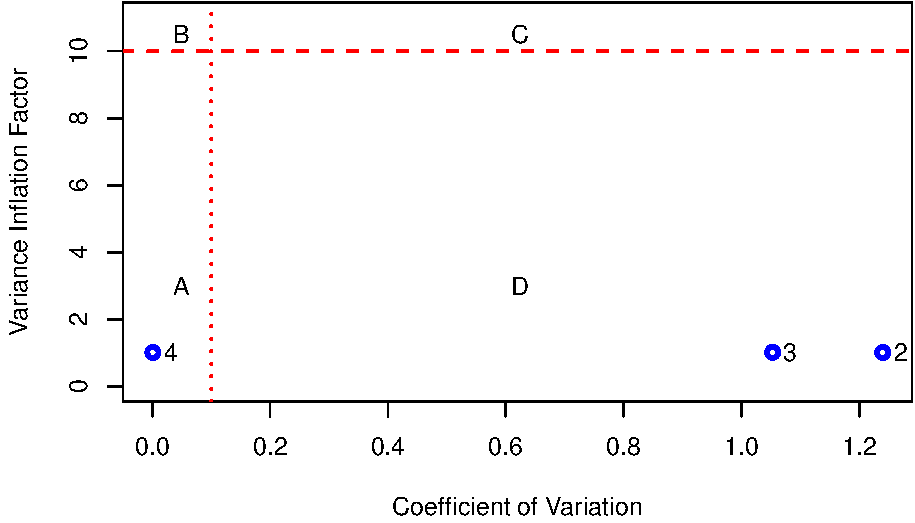
\includegraphics{salmeron-etal_files/figure-latex/FigureS2-1.pdf}
\caption{\label{fig:FigureS2}Representation of the VIFs and CVs of explanatory variables in Simulation 2. A troubling degree of non-essential multicollinearity due to variable 4 is detected by considering thresholds of 0.1002506 (CV) and 10 (VIF) highlighted with red lines.}
\end{figure}

\begin{figure}
\centering
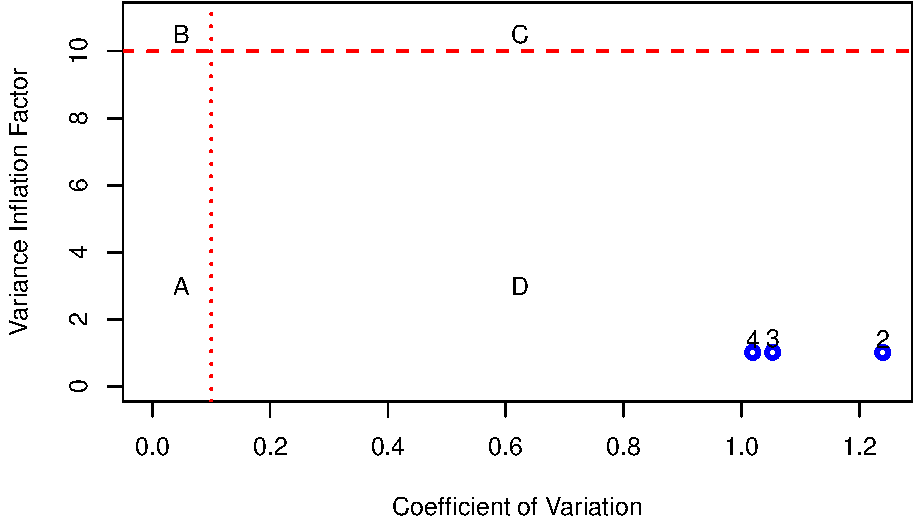
\includegraphics{salmeron-etal_files/figure-latex/FigureS3-1.pdf}
\caption{\label{fig:FigureS3}Representation of the VIFs and CVs of explanatory variables in Simulation 3 . The degree of multicollinearity is not troubling by considering thresholds of 0.1002506 (CV) and 10 (VIF) highlighted with red lines.}
\end{figure}

Analogously, we present Figures \ref{fig:FigureExample1} and \ref{fig:FigureExample2} for Examples 1 and 2, respectively. For Example 1, it is concluded that the only type of troubling multicollinearity is non-essential due to the second variable (\textbf{HIPC}). On the other hand, for Example 2 it is concluded that the only type of troubling multicollinearity is that essentially due to the relationship existing between the third and fourth variables (\textbf{limit} and \textbf{rating}).

\begin{figure}
\centering
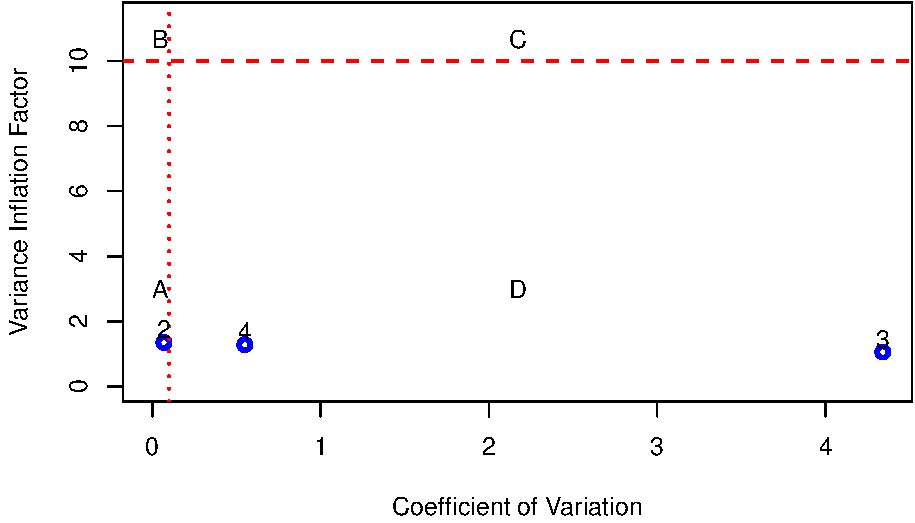
\includegraphics{salmeron-etal_files/figure-latex/FigureExample1-1.pdf}
\caption{\label{fig:FigureExample1}Representation of the VIFs and CVs of the variables of example 1. A troubling degree of non-essential multicollinearity generated by variable 2 (HIPC) by considering thresholds of 0.1002506 (CV) and 10 (VIF) highlighted with red lines.}
\end{figure}

\begin{figure}
\centering
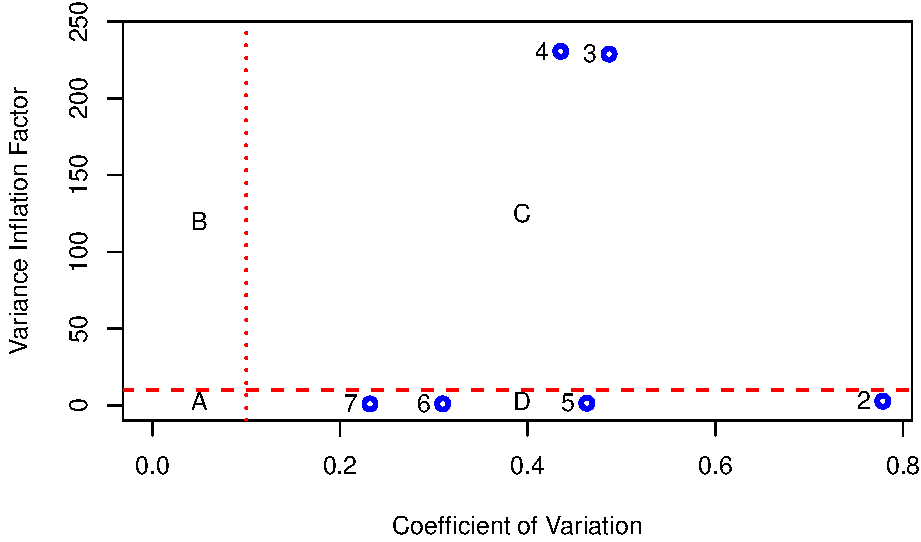
\includegraphics{salmeron-etal_files/figure-latex/FigureExample2-1.pdf}
\caption{\label{fig:FigureExample2}Representation of the VIFs and CVs of the variables of example 2. A troubling degree of Essential multicollinearity generated by variables 3 and 4 (limit and rating) by considering thresholds of 0.1002506 (CV) and 10 (VIF) highlighted with red lines.}
\end{figure}

\hypertarget{summary}{%
\section{Summary}\label{summary}}

This paper analyses the limitations that may arise in detecting the problem of troubling multicollinearity in a linear regression model due to transformations performed on the data. The discussion is used to illustrate that the MC index presented by Lin et al. (2020) depends on the way that the data are transformed.

It was shown that when the \emph{studentise} transformation is performed, the measure is stable for \emph{measuring what variable contributes the most to the linear relationship, and thus identifying what variables best explain the collinearity in the original data} (Lin et al. 2020), as long as the multicollinearity is essential. This kind of transformation was taken as default by the authors and this paper contributes with a formal justification. Note that the MC index only provides interesting information if the troubling multicollinearity is previously detected using other measures (such as the VIF or the CN).

Summarizing, the achievement of the goal intended by the \CRANpkg{mcvis} package is conditioned by the following limitations:

\begin{itemize}
\tightlist
\item
  It is not able to detect non-essential multicollinearity.
\item
  Other measures (as the VIF or CN) should be applied previously to determine whether the degree of essential multicollinearity is troubling.
\item
  The \emph{studentise} transformation should be applied.
\item
  It is not applicable for dummy variables.
\end{itemize}

Finally, it is proposed to use a scatter plot between the VIFs and the CVs, on the one hand, to detect whether the degree of multicollinearity (essential or not essential) is troubling and, on the other hand, to detect which variables are causing the multicollinearity. This would overcome the limitations of the \CRANpkg{mcvis} package discussed above while achieving its overall purpose.

\hypertarget{acknowledgments}{%
\section{Acknowledgments}\label{acknowledgments}}

This work has been supported by project PP2019-EI-02 of the University of Granada (Spain), by project A-SEJ-496-UGR20 of the Andalusian Government's Counseling of Economic Transformation, Industry, Knowledge and Universities (Spain) and by project I+D+i PID2019-107767GA-I0 financed by MCIN/AEI/10.13039/501100011033.

\hypertarget{references}{%
\section{References}\label{references}}

\hypertarget{references-1}{%
\section*{References}\label{references-1}}
\addcontentsline{toc}{section}{References}

\hypertarget{refs}{}
\begin{CSLReferences}{1}{0}
\leavevmode\vadjust pre{\hypertarget{ref-Belsley1991}{}}%
D. Belsley. A guide to using the collinearity diagnostics. \emph{Computational Science in Economics and Manegement}, 4: 33--50, 1991.

\leavevmode\vadjust pre{\hypertarget{ref-Belsley1984}{}}%
D. A. Belsley. Demeaning conditioning diagnostics through centering. \emph{The American Statistician}, 38(2): 73--77, 1984.

\leavevmode\vadjust pre{\hypertarget{ref-Belsleyetal1980}{}}%
D. A. Belsley, E. Kuh and R. E. Welsch. \emph{{Regression diagnostics: Identifying influential data and sources of collinearity}.} New York: John Wiley \& Sons, 1980.

\leavevmode\vadjust pre{\hypertarget{ref-garcia2019claudia}{}}%
C. García, R. Salmerón and C. B. García. Choice of the ridge factor from the correlation matrix determinant. \emph{Journal of Statistical Computation and Simulation}, 89(2): 211--231, 2019.

\leavevmode\vadjust pre{\hypertarget{ref-garciaetal2016}{}}%
J. García, R. Salmerón, C. García and M. López. Standardization of variables and collinearity diagnostic in ridge regression. \emph{International Statistical Review}, 84: 245--266, 2016.

\leavevmode\vadjust pre{\hypertarget{ref-Gujarati2010}{}}%
D. Gujarati. \emph{{Basic Econometrics}.} 8th ed McGraw Hill, 2010.

\leavevmode\vadjust pre{\hypertarget{ref-HalkosTsilika}{}}%
G. Halkos and K. Tsilika. Programming correlation criteria with free cas software. \emph{Computational Economics}, 52(1): 299--311, 2018.

\leavevmode\vadjust pre{\hypertarget{ref-HoerlKennard1970a}{}}%
A. E. Hoerl and R. W. Kennard. Ridge regression: Biased estimation for nonorthogonal problems. \emph{Technometrics}, 12(1): 55--67, 1970.

\leavevmode\vadjust pre{\hypertarget{ref-HastieTibshirani}{}}%
G. James, D. Witten, T. Hastie and R. Tibshirani. \emph{An introduction to statistical learning with application in r.} Springer, 2013.

\leavevmode\vadjust pre{\hypertarget{ref-ISLR}{}}%
G. James, D. Witten, T. Hastie and R. Tibshirani. \emph{ISLR: Data for an introduction to statistical learning with applications in r.} 2021. URL \url{https://CRAN.R-project.org/package=ISLR}. R package version 1.4.

\leavevmode\vadjust pre{\hypertarget{ref-LinWangMueller2020}{}}%
C. Lin, K. Wang and S. Mueller. MCVIS: A new framework for collinearity discovery, diagnostic and visualization. \emph{Journal of Computational and Graphical Statistics}, 2020. DOI \href{https://doi.org/10.1080/10618600.2020.1779729}{10.1080/10618600.2020.1779729}.

\leavevmode\vadjust pre{\hypertarget{ref-Marquardt1970}{}}%
D. W. Marquardt. {Generalized inverses, ridge regression, biased linear estimation and nonlinear estimation}. \emph{Technometrics}, 12(3): 591--612, 1970.

\leavevmode\vadjust pre{\hypertarget{ref-Marquardt1980}{}}%
D. W. Marquardt. You should standardize the predictor variables in your regression models. \emph{J. Amer. Statist. Assoc.}, 75(369): 87--91, 1980.

\leavevmode\vadjust pre{\hypertarget{ref-Novales1988}{}}%
A. Novales. \emph{{Econometría}.} Madrid: McGraw-Hill, 1988.

\leavevmode\vadjust pre{\hypertarget{ref-OBrien2007}{}}%
R. M. O'Brien. {A caution regarding rules of thumb for variance inflation factors}. \emph{Quality \& Quantity}, 41: 673--690, 2007.

\leavevmode\vadjust pre{\hypertarget{ref-ramanathan}{}}%
R. Ramanathan. Introductory econometrics with applications. 2002.

\leavevmode\vadjust pre{\hypertarget{ref-Salmeron2020b}{}}%
R. Salmerón, C. García and J. García. A guide to using the r package multiColl for detecting multicollinearity. \emph{Computational Economics}, 57: 529--536, 2021a. DOI \href{https://doi.org/10.1007/s10614-019-09967-y}{10.1007/s10614-019-09967-y}.

\leavevmode\vadjust pre{\hypertarget{ref-salmeron2019velilla}{}}%
R. Salmerón, C. García and J. García. Comment on {``a note on collinearity diagnostics and centering''} by velilla (2018). \emph{The American Statistician}, 74(1): 68--71, 2020a.

\leavevmode\vadjust pre{\hypertarget{ref-Salmeron2022}{}}%
R. Salmerón, C. García and J. García. The multiColl package versus other existing packages in r to detect multicollinearity. \emph{Computational Economics}, 2021b. DOI \href{https://doi.org/10.1007/s10614-021-10154-1}{10.1007/s10614-021-10154-1}.

\leavevmode\vadjust pre{\hypertarget{ref-salmeron2018JSCS}{}}%
R. Salmerón, C. García and J. García. Variance inflation factor and condition number in multiple linear regression. \emph{Journal of Statistical Computation and Simulation}, 88: 2365--2384, 2018a.

\leavevmode\vadjust pre{\hypertarget{ref-salmeron2018}{}}%
R. Salmerón, J. García, C. García and M. López. Transformation of variables and the condition number in ridge estimation. \emph{Computational Statistics}, 33: 1497--1524, 2018b.

\leavevmode\vadjust pre{\hypertarget{ref-Salmeron2020a}{}}%
R. Salmerón, A. Rodríguez and C. García. Diagnosis and quantification of the non-essential collinearity. \emph{Computational Statistics}, 35: 647--666, 2020b.

\leavevmode\vadjust pre{\hypertarget{ref-SneeMarquardt1984}{}}%
R. D. Snee and D. W. Marquardt. {Comment: Collinearity diagnostics depend on the domain of prediction, the model, and the data}. \emph{The American Statistician}, 38(2): 83--87, 1984.

\leavevmode\vadjust pre{\hypertarget{ref-Tibshirani1996}{}}%
R. Tibshirani. Regression shrinkage and selection via the lasso. \emph{Journal of the Royal Statistical Society. Series B (Methodological)}, 267--288, 1996.

\leavevmode\vadjust pre{\hypertarget{ref-tourr}{}}%
H. Wickham, D. Cook, H. Hofmann and A. Buja. Tourr: A r package for exploring multivariate data with projections. \emph{Journal of Statistical Software}, 40(2): 1--18, 2011. DOI \href{https://doi.org/10.18637/jss.v040.i02}{10.18637/jss.v040.i02}.

\leavevmode\vadjust pre{\hypertarget{ref-Wooldridge2008}{}}%
J. M. Wooldridge. \emph{{Introducción a la econometría. Un enfoque moderno}.} Second Madrid: Thomson Paraninfo, 2008.

\leavevmode\vadjust pre{\hypertarget{ref-ZouHastie}{}}%
H. Zou and T. Hastie. Regularization and variable selection via the elastic net. \emph{Journal of the Royal Statistical Society: Series B (Statistical Methodology)}, 67: 301--320, 2005.

\end{CSLReferences}

\bibliography{salmeron-etal.bib}

\address{%
Roman Salmeron Gomez\\
University of Granada\\%
Department of Quantitative Methods for Economics and Busines\\ Poligono La Cartuja sn, 18071, Granada, Spain.\\
%
\url{http://metodoscuantitativos.ugr.es/pages/web/romansg}\\%
\textit{ORCiD: \href{https://orcid.org/0000-0003-2589-4058}{0000-0003-2589-4058}}\\%
\href{mailto:romansg@ugr.es}{\nolinkurl{romansg@ugr.es}}%
}

\address{%
Catalina B. Garcia Garcia\\
University of Granada\\%
Department of Quantitative Methods for Economics and Busines\\ Poligono La Cartuja sn, 18071, Granada, Spain.\\
%
\url{http://metodoscuantitativos.ugr.es/pages/web/cbgarcia}\\%
\textit{ORCiD: \href{https://orcid.org/0000-0003-1622-3877}{0000-0003-1622-3877}}\\%
\href{mailto:cbgarcia@ugr.es}{\nolinkurl{cbgarcia@ugr.es}}%
}

\address{%
Ainara Rodriguez Sanchez\\
U.N.E.D.\\%
Department of Applied Economics and Economic History\\ Madrid, Spain.\\
%
\url{http://metodoscuantitativos.ugr.es/pages/web/cbgarcia}\\%
\textit{ORCiD: \href{https://orcid.org/0000-0003-1622-3877}{0000-0003-1622-3877}}\\%
\href{mailto:arsanchez@cee.uned.es}{\nolinkurl{arsanchez@cee.uned.es}}%
}

\address{%
Claudia Garcia Garcia\\
Complutense University of Madrid\\%
Department of Applied Economics, Structure and History\\ Madrid, Spain.\\
%
\url{http://metodoscuantitativos.ugr.es/pages/web/cbgarcia}\\%
\textit{ORCiD: \href{https://orcid.org/0000-0003-1622-3877}{0000-0003-1622-3877}}\\%
\href{mailto:clgarc13@ucm.es}{\nolinkurl{clgarc13@ucm.es}}%
}
